\iffalse
\let\negmedspace\undefined
\let\negthickspace\undefined
\documentclass[journal,12pt,twocolumn]{IEEEtran}
\usepackage{cite}
\usepackage{amsmath,amssymb,amsfonts,amsthm}
\usepackage{algorithmic}
\usepackage{graphicx}
\usepackage{textcomp}
\usepackage{xcolor}
\usepackage{txfonts}
\usepackage{listings}
\usepackage{enumitem}
\usepackage{mathtools}
\usepackage{gensymb}
\usepackage{comment}
\usepackage[breaklinks=true]{hyperref}
\usepackage{tkz-euclide} 
\usepackage{listings}
\usepackage{gvv}                            \usepackage{tikz}
\usepackage{circuitikz}
\def\inputGnumericTable{}                                
\usepackage[latin1]{inputenc}                            
\usepackage{color}                                       
\usepackage{array}                                       
\usepackage{longtable}                                   
\usepackage{calc}                              
\usepackage{tikz}
\usepackage{multirow}                                    
\usepackage{hhline}                                      
\usepackage{ifthen}                            
\usepackage{caption}
\usepackage{lscape}
\usepackage{amsmath}
\newtheorem{theorem}{Theorem}[section]
\newtheorem{problem}{Problem}
\newtheorem{proposition}{Proposition}[section]
\newtheorem{lemma}{Lemma}[section]
\newtheorem{corollary}[theorem]{Corollary}
\newtheorem{example}{Example}[section]
\newtheorem{definition}[problem]{Definition}
\newcommand{\BEQA}{\begin{eqnarray}}
\newcommand{\EEQA}{\end{eqnarray}}
\newcommand{\define}{\stackrel{\triangle}{=}}
\theoremstyle{remark}
\newtheorem{rem}{Remark}

\begin{document}

\bibliographystyle{IEEEtran}
\vspace{3cm}

\title{GATE 2022 BM.38}
\author{EE23BTECH11010 - VENKATESH BANDAWAR$^{*}$% <-this % stops a space
}
\maketitle
\newpage
\bigskip
\textbf{Question:} An input $x(t)$ is applied to a system with a frequency transfer function given by
$H(j\omega)$ as shown below. The magnitude and phase response of the transfer function
are shown below. If $y(t_d) = 0$ for $x(t) = u(t)$, the time $t_d (> 0)$ is.\\ 
\hfill(Gate 2022 BM.38)
\begin{figure}[!h] 
\centering
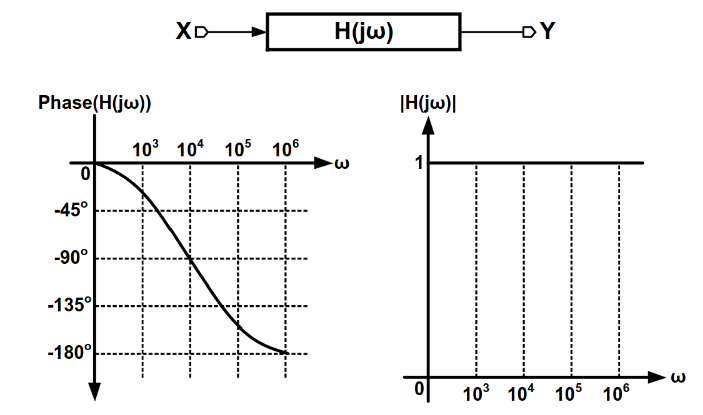
\includegraphics[width=\columnwidth]{2022/BM/38/figs/given_graph.png}
\caption{Graph of y(t)}
\label{fig:Graph1_gate_BM_38}
\end{figure}

\solution 
\fi
\begin{table}[!h]
    \centering
    \begin{tabular}{|c|c|}
\hline
    \textbf{Parameter} & \textbf{Description} \\
    \hline
    $x(t) = u(t)$ & Input signal \\
    \hline
    $y(t)$ & Output signal\\
    \hline
    $X(j\omega)$ & Fourier Transform of $x(t)$\\
    \hline
    $Y(j\omega)$ & Fourier Transform of $y(t)$\\
    \hline
    $H(j\omega) = \frac{Y(j\omega)}{X(j\omega)}$ & Transfer function \\
    \hline
\end{tabular}

    \caption{Input Parameters Table}
\end{table}

% \because \abs{H\brak{f}} &= 1\\
%     \abs{z} &= \abs{\bar{z}}\\
%     \therefore H(f) &= \frac{a - j2\pi f}{a + j2\pi f}\\
from graph \ref{Phase of H(f)2022_bm_38}
\begin{align}
    \angle {H(j\omega)} = -2 \tan^{-1}\brak{\frac{\omega}{a}}
\end{align}
At $\omega = 10^4, \angle{H(j\omega)} = -\frac{\pi}{2}$
\begin{align}
    \implies a = 10^4 
\end{align}
\begin{figure}[!h]
    \centering
    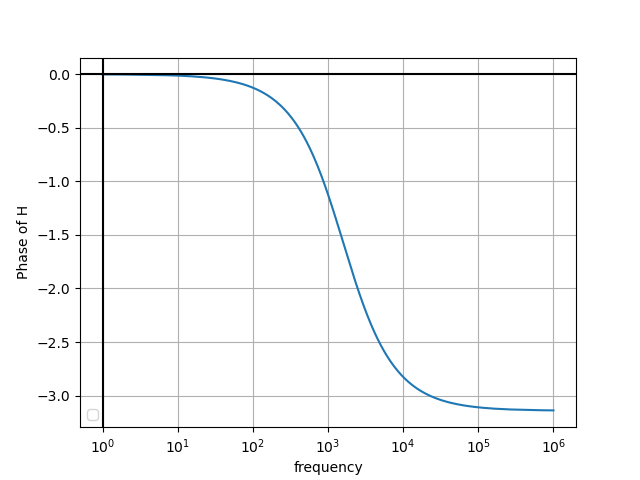
\includegraphics[width=\columnwidth]{2022/BM/38/figs/phase.png}
    \caption{Phase of H(f)}
    \label{Phase of H(f)2022_bm_38}
\end{figure}
\begin{align}
    \angle {H(j\omega)} &= \tan^{-1}\brak{\frac{-\omega}{a}} - \tan^{-1}\brak{\frac{\omega}{a}}\\
    H(j\omega) &= \frac{e^{j\tan^{-1}\brak{\frac{-\omega}{a}}}}{e^{j\tan^{-1}\brak{\frac{\omega}{a}}}}\\
    &= \frac{\frac{a - j\omega}{\sqrt{a^2 + \omega^2}}}{\frac{a + j\omega}{\sqrt{a^2 + \omega^2}}}\\
    &= \frac{a - j\omega}{a + j\omega}
\end{align}
Substitute $s = j\omega$
\begin{align}
    u(t) &\system{\mathcal{L}} \frac{1}{s}\\
    Y(s) &= \frac{1}{s} \frac{a - s}{a + s}\\
    &= \frac{1}{s} - \frac{2}{a + s}\\
    \frac{1}{s} &\mathrel{\substack{\mathcal{L}^{-1}\\\longleftrightarrow}} u(t)\\
    \frac{1}{a + s} &\mathrel{\substack{\mathcal{L}^{-1}\\\longleftrightarrow}} e^{-at} u(t) \\
    y(t) &= (1-2e^{-at}) u(t)
\end{align}
Verification of laplace transform:
\begin{figure}[!h]
    \centering
    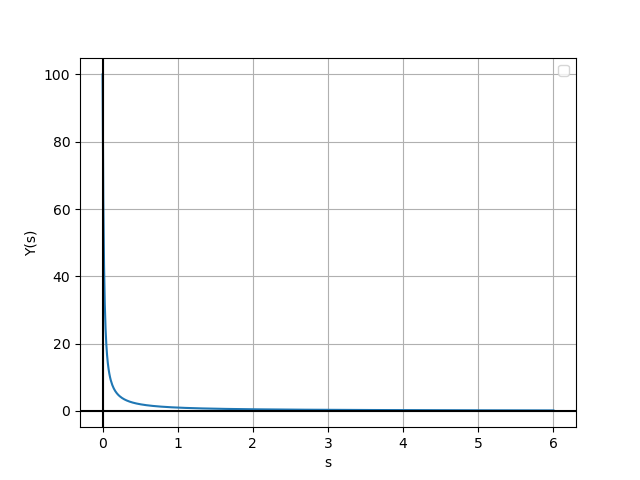
\includegraphics[width=\columnwidth]{2022/BM/38/figs/laplace_transform1.png}
    \caption{Laplace Transform of $u(t)$}
\end{figure}
\begin{figure}[!h]
    \centering
    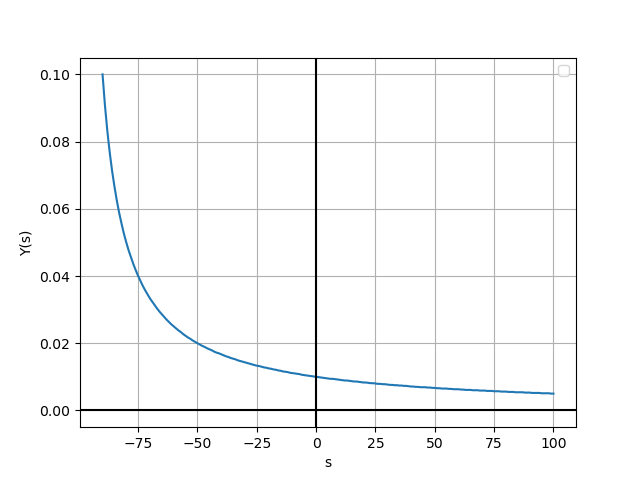
\includegraphics[width=\columnwidth]{2022/BM/38/figs/laplace_transform2.png}
    \caption{Laplace Transform $of e^{-at} u(t)$}
\end{figure}
\begin{align}
    \because y(t_d) &= 0 \\
    t_d &= 100 \ln{2} \micro s 
\end{align}
\begin{figure}[!h]
    \centering
    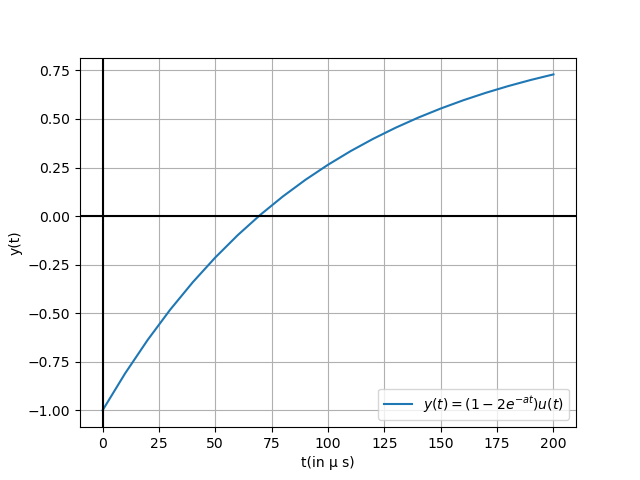
\includegraphics[width=\columnwidth]{2022/BM/38/figs/graph.png}
\end{figure}

